% thesis.tex
%
% This file is root file for an example thesis written using the
% IIT Bombay LaTeX Style file.
% Created by Amey Karkare (21 June 2007)
%
% It is provided without warranty on an AS IS basis.

%=====================================================================
% Read: http://www.cse.iitb.ac.in/karkare/iitbthesis/
%    FAQ.txt     for frequently asked quetions
%    Changes.txt for changes
%    README      for more information
%=====================================================================

%=====================================================================
% DOCUMENT STYLE
%=====================================================================
% IITB PhD Thesis format default settings are:
%   12pt, one-sided printing on a4 size paper
\documentclass[openright,twoside]{iitkthesis}
% For two-sided printing, with Chapter starting on odd-numbered pages,
% use the following line instead:  
%%\documentclass[openright,twoside]{iitbthesis}

%=====================================================================
% OPTIONAL PACKAGES
%=====================================================================
% To include optional packages, use the \usepackage command.
% For e.g., The package epsfig is used to bring in the Encapsulated
%    PostScript figures into the document.
%    The package times is used to change the fonts to Times Roman;
%=====================================================================

%=====================================================================
%  Single counter for theorems and theorem-like environments:
%=====================================================================
\newtheorem{theorem}{Theorem}[chapter]
\newtheorem{assertion}[theorem]{Assertion}
\newtheorem{claim}[theorem]{Claim}
\newtheorem{conjecture}[theorem]{Conjecture}
\newtheorem{corollary}[theorem]{Corollary}
\newtheorem{definition}[theorem]{Definition}
\newtheorem{example}[theorem]{Example}
\newtheorem{figger}[theorem]{Figure}
\newtheorem{lemma}[theorem]{Lemma}
\newtheorem{prop}[theorem]{Proposition}
\newtheorem{remark}[theorem]{Remark}

\usepackage{minted}
\usemintedstyle{bw}

\usepackage{fontspec}
\setmonofont[Scale=0.85]{DejaVu Sans Mono}

\usepackage[sorting=none, maxbibnames=99, minbibnames=99]{biblatex}
\bibliography{citations}
\usepackage{amsmath}
\usepackage{lipsum}
\usepackage{float}
\usepackage[hidelinks]{hyperref}
\usepackage{microtype}
\usepackage[font=small,labelfont=bf]{caption}
\usepackage{fancyref}
\usepackage{color,soul} % for highlights
\usepackage{enumerate}
\usepackage{tabularx}

\setlength{\headheight}{15pt}

\expandafter\def\csname PY@tok@err\endcsname{}

\floatstyle{ruled}
\newfloat{program}{thp}{lop}
\floatname{program}{Figure}

\numberwithin{program}{chapter}

\BeforeBeginEnvironment{program}{\begin{singlespace}}
\AfterEndEnvironment{program}{\end{singlespace}}

%=====================================================================
% End of Preamble, start of document
%

\begin{document}

%=====================================================================
% Include the prelude for Title page, abstract, table of contents, etc
% You need to modify it to contain your details
% prelude.tex
%   - titlepage
%   - dedication (optional)
%   - approval sheet
%   - course certificate
%   - table of contents, list of tables and list of figures
%   - nomenclature
%   - abstract
%============================================================================


\clearpage\pagenumbering{roman}  % This makes the page numbers Roman (i, ii, etc)



% TITLE PAGE
%   - define \title{} \author{} \date{}
\title{Functional SMT solving: A new interface for programmers}
\author{Siddharth Agarwal}
\date{June, 2012}

%  - Roll number, required for title page, approval sheet, and
%    certificate of course work 
\rollnum{Y7027429} 

%   - The default degree is ``Doctor of Philosophy''
%     (unless the document style msthesis is specified
%      and then the default degree is ``Master of Science'')
%     Degree can be changed using the command \iitbdegree{}
\iitbdegree{Master of Technology}

%   - The default report type is preliminary report.
%      * for a PhD thesis, specify \thesis
\thesis
%      * for a M.Tech./M.Phil./M.Des./M.S. dissertation, specify \dissertation
%\dissertation
%      * for a DIIT/B.Tech./M.Sc.project report, specify \project
%\project
%      * for any other type, use  \reporttype{}
%\reporttype{ReportType}

%   - The default department is ``Unknown Department''
%     The department can be changed using the command \department{}
\department{Computer Science \& Engineering}

%    - Set the guide's name
\setguide{Prof Amey Karkare}
\setguidedept{Department of Computer Science \& Engineering}

%   - once the above are defined, use \maketitle to generate the titlepage
\maketitle

%--------------------------------------------------------------------%
% CERTIFICATE
%     The first page after the title page.
\makecertificate

%--------------------------------------------------------------------%
% COPYRIGHT PAGE
%   - To include a copyright page use \copyrightpage
% \copyrightpage

%--------------------------------------------------------------------%
% ABSTRACT
\begin{abstract}
Satisfiability Modulo Theories (SMT) solvers are powerful tools that can quickly solve
complex constraints involving booleans, integers, first-order logic
predicates, lists, and other data types. They have a vast number of potential
applications, from constraint solving to program analysis and verification.
However, they are so complex to use that their power is inaccessible to all
but experts in the field.

We present an attempt to make using SMT solvers simpler by integrating the Z3 solver
into a host language, Racket. Our system defines a programmer's interface in
Racket that makes it easy to harness the power of Z3 to discover solutions to
logical constraints. The interface, although in Racket, retains the
structure and brevity of the SMT-LIB format. We demonstrate this using a range
of examples, from simple constraint solving to verifying recursive functions, all in
a few lines of code.
\end{abstract}

%--------------------------------------------------------------------%
% DEDICATION
%   Dedications, if any.
\begin{dedication}
To my grandfather
\end{dedication}

% Acknowledgements
\begin{acknowledgments}

This project would have never have even been started had it not been for my
thesis advisor Dr Amey Karkare's help and guidance. Right from the time we
were looking for ideas to when we finally had a concrete proposal in hand, his
support has been invaluable. He entertained all my crazy ideas, found which
ones had merit, and helped me build on them. I wouldn't have been able to do
this without him.

I'd like to thank my parents and the others in my life for being patient with
me, especially towards the final stretch of thesis completion when I wasn't at
my best socially.

The Racket community, at \texttt{\#racket} on Freenode IRC, helped me
understand some of the Racket syntax model's intricacies. That helped me avoid
dead ends both early on and towards the end.

Special thanks to Leonardo de Moura at Microsoft Research for taking the time
out to answer a few questions about Z3.

\end{acknowledgments}

%--------------------------------------------------------------------%
% CONTENTS, TABLES, FIGURES
\tableofcontents
\listoftables

\cleardoublepage
\phantomsection \label{listoffig}
\addcontentsline{toc}{chapter}{List of Figures}
\listof{program}{List of Figures}
%\listoffigures

\cleardoublepage\pagenumbering{arabic} % Make the page numbers Arabic (1, 2, etc)


%=====================================================================
% Include the technical part of the report
%% \include{chap_intro}             % Chapter 1: Introduction
%% \include{chap_others}            % Other chapters as required
%% \include{chap_conclusions}       % Finally the summary & conclusions

%=====================================================================
% APPENDIX
%  Appendices, if any, must precede the cited literatures.
%  Appendices shall be numbered in Roman Capitals (e.g. Appendix IV)

%% \appendix
%% \include{appendix_something}          

%=====================================================================
% PUBLICATIONS
%  publications if any may be listed after the literature cited.
%% \include{mypubs}

%=====================================================================
% ACKNOWLEDGMENTS
%   This is the last item in the thesis. It should be signed by
%   author, with date.


\chapter{Introduction: Satisfiability solvers and interfaces}
\label{chap:intro}

The Boolean satisfiability or SAT problem asks: \textit{Given a boolean
formula with a set of variables in it, is there a way to assign each variable
a value such that the formula becomes true?} The SAT problem is one of the
cornerstones of computer science, with enormous theoretical and practical
implications. Indeed, it was the very first problem to be proved
\textit{NP-complete}~\cite{sat-npcomplete}.

Yet, interest in efficiently solving so-called ``natural'' or ``real-world''
instances of SAT has remained. This is at least partly because a large number
of practical problems are also NP-complete and can be \textit{reduced} to SAT.
Here \textit{reduced} is as it is defined in~\cite{karp21}: roughly, can an
instance of the problem be turned into a boolean formula decided by SAT that's
at most polynomially larger?

\section{Solving SAT: DPLL}

Solving SAT is generally restricted to boolean formulas in conjunctive normal
form (CNF), which consists of \textit{clauses} of boolean
\textit{literals}\footnote{The word \textit{literal} has two different
technical meanings: in computer science, it represents a fixed value such as
the number \texttt{1} or the string \texttt{"Hello"}. In mathematical logic,
it means either an atom (variable: $p$) or its negation ($\neg p$). We use it
here in this latter sense.} joined together with the OR operation ($\vee$),
and these clauses joined together with the AND operation ($\wedge$). It is
proved that the SAT problem for any boolean formula can be reduced to the SAT
problem for formulas in CNF~\cite{karp21}.

CNF formulas have useful properties, such as that they can be represented as a
set of clauses, that at any point a clause once satisfied (shown to be true)
can be dropped from the set, and that showing even one of the clauses to be
false is enough to show that the formula cannot be satisfied.

The simplest way to solve SAT is with a basic backtracking algorithm
(\Fref{fig:sat-backtracking}). The algorithm's recursive nature means it takes
exponential time in the worst case.

\begin{program}

\caption[A na\"{i}ve backtracking algorithm for SAT in Racket]
{A na\"{i}ve backtracking algorithm for SAT in Racket.
\texttt{substitute} substitutes the given value for the atom in the boolean
formula, and returns an updated formula or \texttt{\#f}}

\label{fig:sat-backtracking}
\begin{minted}{scheme}
; atoms is a list of variables to satisfy
(define (solve-sat atoms formula)
  (if (empty? atoms)
      #t   ; no more atoms to substitute means SAT
      (let*
       ([atom (car atoms)]    ; pick the first atom
        [rest-atoms (cdr atoms)]
        [subst-true (substitute formula atom #t)]
        [subst-false (substitute formula atom #f)])

        (or (and subst-true (solve-sat rest-atoms subst-true))
            (and subst-false (solve-sat rest-atoms subst-false))))))
\end{minted}
\end{program}

There are two key insights that can be made here:

\begin{enumerate}

\item \textbf{Unit propagation, or the one-literal clause rule.} \textit{If a
clause contains just one literal, that literal has to be true.} For example,
consider the set of clauses $\{a, a \vee b, \neg a \vee \neg c, b \vee c \vee
d\}$. Since all the clauses need to be true, $a$ must be true. Letting this
happen, we see that $a \vee b$ is true so it is dropped, and $\neg a \vee \neg
c$ simply becomes $\neg c$, which means we are left with the clauses $\{\neg
c, b \vee c \vee d\}$.

At this point unit propagation can be applied once again on $c$, setting it to
false. We are finally left with just the one clause $\{b \vee d\}$.

\item \textbf{Pure literal elimination, or the affirmative-negative rule.}
\textit{If the occurrences of a given variable $p$ are either all $p$ (or all
$\neg p$), then $p$ can be assigned true (or false).} Consider the following
set of clauses: $\{a \vee b, a \vee c, b \vee c \vee \neg d, \neg b \vee \neg
c \vee d\}$. Since $a$ always appears in its positive form, we can assign $a$
true without needing to consider the case where $a$ is false. Thus any clause
that contains $a$ is satisfied and can be dropped. We are left with $\{b \vee
c \vee \neg d, \neg b \vee \neg c \vee d\}$.

\end{enumerate}

The backtracking algorithm, plus these two insights applied at each step, form
the Davis-Putnam-Logemann-Loveland (DPLL) algorithm~\cite{dpll1,dpll2}. The
DPLL algorithm, although over fifty years old, is tremendously successful and
forms the core of many modern complete SAT solvers\footnote{A
\textit{complete} SAT solver is one where a definitive answer is returned,
whether a formula is satisfiable or not. There are also \textit{incomplete}
SAT solvers which return an answer if the formula is satisfiable but do not
return one if it is not. Examples include GSAT and WalkSat~\cite{walksat}.},
including Chaff~\cite{chaff}, GRASP~\cite{grasp} and MiniSat~\cite{minisat}.

Of course, modern SAT solvers employ a large number of heuristic and
optimisation tricks to speed things up. They are highly efficient for
``real-world'' problems and are used in a wide variety of computer science fields,
from automated planning for robots or unmanned vehicles (via the
\textit{satplan} method~\cite{satplan}), to dependency resolution in Linux
package managers such as Zypper~\cite{zypper}. They have also been heavily used in 
program analysis and verification, which is what brings us to the next section.

\section{SMT and DPLL(T): SAT with a twist}

Typically, program analysis tools that used SAT solvers would have to find a
way to translate variables found in programs to boolean ones. For example, a
32-bit integer could be encoded as a set of 32 boolean variables\footnote{It
is also possible to represent integers as boolean variables via predicate
abstraction~\cite{slam}, which is more efficient but potentially loses
information.}.

It was soon realised that pushing this step into the SAT solver would help.
Since users would still be asking whether formulas were satisfiable, except
with variables from more complex domains or \textit{theories}, this approach
was dubbed Satisfiability Modulo Theories (SMT). Early SMT methods
(e.g.~\cite{proc-verification,uclid}) \textit{eagerly} simply converted formulas to
Boolean variables before handing them over to a SAT solver.

Alternatively, one could substitute placeholder boolean variables for theory
variables, supply this \textit{faux} boolean formula to a modified SAT solver,
and write a separate program called a \textit{T-solver} that interacts
\textit{on demand} with the SAT solver to deal with theory variables. The
modified DPLL algorithm is called \textbf{DPLL(T)}~\cite{dpllt:04}, and this
\textit{lazy} approach turns out to be far more efficient than eager methods.
(For a more detailed description of eager and lazy SMT,
see~\cite[Section~3.2]{abstract-dpll}).

State-of-the-art SMT solvers like Z3~\cite{z3}, Yices~\cite{yices} and
CVC3~\cite{cvc3} are based on DPLL(T). They allow users to specify constraints
over booleans, integers, real numbers, arrays, lists, trees, first-order
predicates and other kinds of variables. They either come up with assignments
that satisfy these constraints, or, if possible, a proof that the constraints
aren't satisfiable. SMT solvers have been used to solve problems in planning
and scheduling, program analysis~\cite{Gulwani:08}, whitebox fuzz
testing~\cite{Godefroid:08} and bounded model checking~\cite{Armando:09}.

\section{Using SMT solvers}
\label{sec:usingsmt}

After coming to know of the power SMT solvers have, the first question the
intrepid programmer would ask is how to use one. Unfortunately, the standard
way for programs to interact with SMT solvers is via powerful but relatively
arcane C APIs that require the users to know the particular solver's
internals. For example, \Fref{fig:c-prop} lists a C program that asks Z3
whether the simple proposition $p \wedge \neg p$ is satisfiable.

\begin{program}
\caption{A C program to ask Z3 whether $p \wedge \neg p$ is satisfiable}
\label{fig:c-prop}
\begin{minted}{c}
Z3_config cfg = Z3_mk_config();
Z3_context ctx = Z3_mk_context(cfg);
Z3_del_config(cfg);
Z3_sort bool_sort = Z3_mk_bool_sort(ctx);

Z3_symbol symbol_p = Z3_mk_int_symbol(ctx, 0);

Z3_ast p = Z3_mk_const(ctx, symbol_p, bool_sort);
Z3_ast not_p = Z3_mk_not(ctx, p);

Z3_ast args[2] = {p, not_p};
Z3_ast conjecture = Z3_mk_and(ctx, 2, args);

Z3_assert_cnstr(ctx, conjecture);

Z3_lbool sat = Z3_check(ctx);

Z3_del_context(ctx);
return sat;
\end{minted}
\end{program}

Simultaneously, most SMT solvers also feature interaction via the standard
input language SMT-LIB~\cite{smtlib2:10}. SMT-LIB is \textit{significantly}
easier to use in isolation. The same program in SMT-LIB would look something
like \Fref{fig:smtlib-prop}.

\begin{program}
\caption{An SMT-LIB program to check whether $p \wedge \neg p$ is satisfiable}
\label{fig:smtlib-prop}
\begin{minted}{scheme}
; Declare a variable we don't know the value of yet
(declare-fun p () Bool)
; Try to find a value satisfying a contradiction
(assert (and p (not p)))
(check-sat)
; Prints "unsat", meaning "unsatisfiable"
\end{minted}
\end{program}

The complexity of the C interface keeps going up as we move to less trivial
assertions. \Fref{fig:c-simultaneous} is a C program that asks Z3 to solve the
two simultaneous equations $2x\,+\,3y = 5, 4x\,+\,5y = 7$. (The solution is $x =
-2, y = 3$.)

\begin{program}
\caption{A C program to ask Z3 to solve two simultaneous linear equations}
\label{fig:c-simultaneous}
\begin{minted}{c}
Z3_config cfg = Z3_mk_config();
Z3_set_param_value(cfg, "MODEL", "true");
Z3_context ctx = Z3_mk_context(cfg);
Z3_del_config(cfg);

Z3_sort int_sort = Z3_mk_int_sort(ctx);

Z3_symbol symbol_x = Z3_mk_int_symbol(ctx, 0);
Z3_symbol symbol_y = Z3_mk_int_symbol(ctx, 1);

Z3_ast x = Z3_mk_const(ctx, symbol_x, int_sort);
Z3_ast y = Z3_mk_const(ctx, symbol_x, int_sort);
Z3_ast num2 = Z3_mk_int(ctx, 2, int_sort);
Z3_ast num3 = Z3_mk_int(ctx, 3, int_sort);
Z3_ast num4 = Z3_mk_int(ctx, 4, int_sort);
Z3_ast num5 = Z3_mk_int(ctx, 5, int_sort);
Z3_ast num7 = Z3_mk_int(ctx, 7, int_sort);

Z3_ast eq1 = Z3_mk_eq(ctx, Z3_mk_add(ctx, Z3_mk_mul(ctx, num2, x),
                                          Z3_mk_mul(ctx, num3, y)),
                           num5);
Z3_ast eq2 = Z3_mk_eq(ctx, Z3_mk_add(ctx, Z3_mk_mul(ctx, num4, x),
                                          Z3_mk_mul(ctx, num5, y)),
                           num7);

Z3_assert_cnstr(ctx, eq1);
Z3_assert_cnstr(ctx, eq2);

Z3_model m;
Z3_lbool sat = Z3_check_and_get_model(ctx, &m);

// Z3_L_TRUE means satisfied
if (sat == Z3_L_TRUE) {
  Z3_ast xsolved, ysolved;
  // Omitting some error checking
  Z3_eval(ctx, m, x, &xsolved);
  Z3_eval(ctx, m, x, &ysolved);
  int xval, yval;
  Z3_get_numeral_int(ctx, xsolved, &xval);
  Z3_get_numeral_int(ctx, xsolved, &yval);
  printf("x = %d, y = %d", xval, yval);
}
else {
  printf("No solution to equations");
}
\end{minted}
\end{program}

The SMT-LIB interface is still remarkably brief, though (\Fref{fig:smtlib-simultaneous}).

\begin{program}
\caption{SMT-LIB code to solve two simultaneous linear equations}
\label{fig:smtlib-simultaneous}
\begin{minted}{scheme}
(declare-fun x () Int)
(declare-fun y () Int)
(assert (= (+ (* 2 x) (* 3 y)) 5))
(assert (= (+ (* 4 x) (* 5 y)) 7))
(check-sat)
(eval x)
(eval y)
\end{minted}
\end{program}

However, the SMT-LIB interfaces are generally hard to use directly from C
programs and often not as full-featured\footnote{Z3, for instance, supports
plugging in external theories via the C API, but not via the textual SMT-LIB
interface.}  or extensible. Importantly, it is difficult to write programs
that \textit{interact} with the solver in some way, for example by adding
assertions based on generated models. This makes it difficult to build new
abstractions to enhance functionality.

\subsection*{Summary}

In this chapter, we saw what SAT and SMT solvers are, how they work, and the
power that they have. We also saw why few programmers use SMT solvers now,
instead preferring to hand-code cumbersome search and backtracking algorithms.

\chapter{A new interface: \texttt{z3.rkt}}

In \Fref[plain]{chap:intro}, we demonstrated how cumbersome SMT solvers are to
use. Indeed, we faced the same issues while exploring novel methods to verify,
debug and test functional programs. It felt like the C interface was
hamstringing us, and the SMT-LIB interface was good for basic explorations but
not anything more complicated.

We decided to attempt to solve this: our goal was to implement an SMT-LIB-like
interface in a way that allowed for the same power as the C interface while
appearing naturally integrated into a host language. Since SMT-LIB is {\em
s-expression}-based, for the host language a Lisp dialect was a natural
choice. We chose Microsoft Research's Z3~\cite{z3} as our SMT solver, and
Racket~\cite{racket}, a popular dialect of Scheme~\cite{scheme-r5rs,scheme-r6rs},
for our implementation. We call our implementation \textbf{\texttt{z3.rkt}}. Racket has
extensive facilities for implementing new languages~\cite{Tobin-Hochstadt:11},
not just for the interface to the solver, but also for the resulting tools
that the solver would make possible.

Using this system, the program to check whether a contradiction is satisfiable
(\Fref{fig:rkt-prop}) becomes almost as brief as the SMT-LIB version. The
program to solve two simultaneous linear equations (\Fref{fig:rkt-simultaneous}) is
similarly brief.

\begin{program}
\caption{Using \texttt{z3.rkt} to determine whether $p \wedge \neg p$ is satisfiable}
\label{fig:rkt-prop}
\begin{minted}{scheme}
(smt:with-context
 (smt:new-context)
 (smt:declare-fun p () Bool)
 (smt:assert (and/s p (not/s p)))
 (smt:check-sat))
\end{minted}
\end{program}

\begin{program}
\caption{Solving simultaneous linear equations with \texttt{z3.rkt}}
\label{fig:rkt-simultaneous}
\begin{minted}{scheme}
(smt:with-context
 (smt:new-context)
 (smt:declare-fun x () Int)
 (smt:declare-fun y () Int)
 (smt:assert (=/s (+/s (*/s 2 x) (*/s 3 y)) 5))
 (smt:assert (=/s (+/s (*/s 4 x) (*/s 5 y)) 7))
 (smt:check-sat)
 (values (smt:eval x) (smt:eval y)))
\end{minted}
\end{program}

\section{Interactive SMT solving: two examples}
\label{sec:interactive}

To demonstrate the value in integrating a language with an SMT solver, we turn
our attention to a pair of classic logical puzzles.

\subsection{Sudoku}

A Sudoku puzzle asks the player to complete a partially pre-filled 9$\times$9
grid with the numbers 1 through 9 such that no row, column, or 3$\times$3 box
has two instances of a number. This is a classic constraint satisfaction
problem, and any constraint solver can handle it with ease.

\Fref{fig:sudoku} lists a Racket program using \texttt{z3.rkt} to solve Sudoku.

\begin{program}
\caption{Racket code using \texttt{z3.rkt} to solve Sudoku}
\label{fig:sudoku}
\begin{minted}{scheme}
(define (solve-sudoku grid)
  (smt:with-context
   (smt:new-context)
   ; Declare a scalar datatype (finite domain type) with 9 entries
   (smt:declare-datatypes ()
     ((Sudoku S1 S2 S3 S4 S5 S6 S7 S8 S9)))
   ; Represent the grid as an array from integers to this type
   (smt:declare-fun sudoku-grid () (Array Int Sudoku))
   ; Assert the standard grid rules (row, column, box)
   (add-sudoku-grid-rules)
   ; Add pre-filled entries
   (add-grid grid)
   (define sat (smt:check-sat))
   ; 'sat means we found a solution, 'unsat means we didn't
   (if (eq? sat 'sat)
       ; Retrieve the values from the model
       (for/list ([x (in-range 0 81)])
         (smt:eval (select/s sudoku-grid x)))
       #f)))
\end{minted}
\end{program}

Here we omit a couple of function definitions: \texttt{add-sudoku-grid-rules}
asserts the standard Sudoku grid rules, and \texttt{add-grid} reads a
partially filled grid in a particular format and creates assertions based on
it. We note that the function \texttt{(select/s arr x)} retrieves the value at
\texttt{x} from the array \texttt{arr}, and that this can be used to add
constraints on the array (for instance, \texttt{(smt:assert (=/s (select/s arr
x) y))}). We also note that if a set of constraints is satisfiable, Z3 can
generate a \textit{model} showing this; values can be extracted out of this
model using the \texttt{smt:eval} command.

However, simply finding a solution isn't enough for a good Sudoku solver: it
must also verify that there aren't any other solutions. The usual way to do
that for a constraint solver is by retrieving a generated model, adding
assertions such that this model cannot be generated again, and then asking the
solver whether the system of assertions is still satisfiable. If it is, a
second solution exists and the puzzle is considered invalid.

In such situations, the interactivity offered by \texttt{z3.rkt} becomes
useful: it lets the programmer add dynamically discovered constraints on the
fly. The last part of the solution might then become something like
\Fref{fig:sudoku-unique}.

\begin{program}
\caption{Ensuring that a Sudoku grid has exactly one solution}
\label{fig:sudoku-unique}
\begin{minted}{scheme}
   ...
   (if (eq? sat 'sat)
       ; Make sure no other solution exists
       (let ([result-grid
         (for/list ([x (in-range 0 81)])
           (smt:eval (select/s sudoku-grid x)))])
         ; Assert that we want a brand new solution by
         ; asserting (not <current solution>)
         (smt:assert
          (not/s (apply and/s
                   (for/list ([(x i) (in-indexed result-grid)])
                     (=/s (select/s sudoku-grid i) x)))))
         (if (eq? (smt:check-sat) 'sat)
             #f ; Multiple solutions
             result-grid))
       #f)))
\end{minted}
\end{program}

This part can even be abstracted out into a function that returns a
lazily-generated sequence of satisfying assignments for any given set of
constraints.

\subsection{Number Mind}

The deductive game Bulls and Cows, commercialised as
Master~Mind~\cite{mastermind}, is popular all around the world. The rules may
vary slightly, but their essence stays the same: Two players play the game.
One player (we'll call her Alice) thinks of a 4-digit number, and the other
(Bob) tries to find it. Bob guesses a number, and Alice tells him how many
digits he has correct and in the correct position (\textit{bulls}) and how
many he has correct but in the wrong position (\textit{cows}). Through
repeated guessing Bob tries to arrive at the answer.

The game is deceptively simple: while even the standard 4-digit variant is
challenging for humans, the general problem for $n$ digits is
NP-complete~\cite{mastermindnpc}. As such, it becomes an interesting problem for
constraint solvers.

For simplicity, we tackle a variant of the game:
Number~Mind~\cite{numbermind}, where Bob only tells Alice how many digits are
correct and in the correct place (bulls). The user is Alice and the computer
Bob, which means that the game is \textit{interactive}. An API to solve
Number~Mind would have

\begin{enumerate}[(a)]
\item a way to tell the computer how many digits the number has
\item a way for the computer to guess a number
\item a way for the user to tell the computer how many digits it got correct
  in the last guess.
\end{enumerate}

The constraint solver would have an important role in not just (a) and (c) but
also (b), since we would like the computer to make ``reasonable" guesses and
not just wild ones. We do this by never guessing a number that would be
impossible because of the answers already given.

Our system makes all three tasks simple. \Fref{fig:numbermind} defines three
functions, each corresponding to one of the tasks above.

\begin{program}
\caption{Solving Number Mind using \texttt{z3.rkt}}
\label{fig:numbermind}
\begin{minted}{scheme}
; (a) Create variables for each digit
(define (make-variables num-digits)
  (define vars (smt:make-fun/list num-digits () Int))
  ; Every variable is between 0 and 9
  (for ([var vars]) (smt:assert (and/s (>=/s var 0) (<=/s var 9))))
  vars)

; (b) Guess a number. Returns the guess as a list of digits,
; or #f meaning no number can satisfy all the constraints.
(define (get-new-guess vars)
  (define sat (smt:check-sat))
  (if (eq? sat 'sat)
      ; Get a guess from the SMT solver
      (map smt:eval vars)
      #f))

; (c) How many digits the computer got correct. If a digit is
; correct then we assign it the value 1, otherwise 0. We sum up
; the values and assert that that's equal to the number of correct
; digits.
(define (add-guess vars guess correct-digits)
  (define correct-lhs
    (apply +/s
           (for/list ([x guess]
                      [var vars])
             (ite/s (=/s var x)
                    1      ; Correct guess
                    0))))  ; Wrong guess
  (smt:assert (=/s correct-lhs correct-digits)))
\end{minted}
\end{program}

As a demonstration of \texttt{z3.rkt}, we have written a small web application
around the code. The web application is available at

\begin{center}
\url{http://numbermind.less-broken.com}
\end{center}

The source is also available:

\begin{center}
\url{https://github.com/sid0/numbermind}
\end{center}

\section{Design and implementation}
\label{sec:design-impl}

\texttt{z3.rkt} is currently implemented as a few hundred lines of Racket code
that interface with the Z3 engine via the provided library. Since the system is
still a work in progress, some of these details might change in the future.

\subsubsection{The Z3 wrapper.} We use Racket's foreign interface \cite{racket/foreign}
to map the Z3 library's C functions into Racket. The programmer interface
communicates with Z3 by calling the Racket functions defined by the
wrapper. While it is possible to use the Z3 wrapper directly, we highly
recommend using the programmer interface instead.

\subsubsection{Built-in functions.} Z3 comes with a number of built-in functions that
operate on booleans, numbers, and more complex values. We expose these
functions directly but add a \texttt{/s} suffix to their usual names in the
SMT-LIB standard, because most SMT-LIB names are already defined as functions
by Racket and we want to avoid colliding with them.

\subsubsection{The core commands.} This is a small set of Racket macros and
functions layered on top of the Z3 wrapper. The aim here is to hide the
complexities of the C wrapper (as discussed in \Fref[plain]{sec:usingsmt}) and
stay as close to SMT-LIB version 2 commands \cite{smtlib2:10} as possible. We
prefix commands with \texttt{smt:} to avoid collisions with Racket functions.

\subsection{Derived abstractions}
\label{sec:derived}

Since the full power of Racket is available to us, we can define abstractions
that allow users to simplify their code. For example, SMT-LIB allows users to
define macros via the \texttt{define-fun} command, as demonstrated by
\Fref{fig:smtlib-max}.

\begin{program}
\caption{An SMT-LIB macro, defined with \texttt{define-fun}}
\label{fig:smtlib-max}
\begin{minted}{scheme}
(define-fun max ((a Int) (b Int)) Int
  (ite (> a b) a b)) ; ite is short for if-then-else
...
(assert (= (max 4 7) 7))
\end{minted}
\end{program}

However, Z3's API exposes no such command. Our first attempt was to define a
Racket function to do the same thing, as in \Fref{fig:rkt-max-fn}.

\begin{program}
\caption{A first attempt at ``macros" in \texttt{z3.rkt}}
\label{fig:rkt-max-fn}
\begin{minted}{scheme}
(define (smt-max a b)
  (ite/s (>/s a b) a b))
...
(smt:assert (=/s (smt-max 4 7) 7))
\end{minted}
\end{program}

This works for smaller macros like \texttt{max}, but in our experience this
sort of na\"{i}ve substitution can result in final expressions for deeply
nested functions becoming too large for Z3 to handle\footnote{In theory, we
could merge common parts of expressions to reduce the number of AST nodes
generated. In our experiments, this proved to be effective, yet still
significantly slower than the solution we finally adopted.}.

We note, however, that any macro can also be written as a universally
quantified formula. For example, \texttt{max} can be rewritten as shown in
\Fref{fig:max-forall}.

\begin{program}
\caption{Macros as universally quantified formulas}
\label{fig:max-forall}
\begin{minted}{scheme}
(declare-fun max (Int Int) Int)
(assert (forall ((a Int) (b Int))
                (= (max a b)
                   (ite (> a b) a b))))
\end{minted}
\end{program}

Indeed, Z3 has a \textit{macro finder} component that identifies and
eliminates universal quantifiers that are macros in disguise. We finally
solved the problem by providing a Racket macro, \texttt{smt:define-fun}, that
has the same syntax as the SMT-LIB command and that performs precisely this
transformation.

The definition of \texttt{smt:define-fun} is listed in \Fref{fig:define-fun}.
We use Scheme's \texttt{syntax-rules} macro system \cite[Section~4.3.2]{scheme-r5rs}
to its fullest extent. \texttt{syntax-rules} accepts pairs of input and output
patterns and goes with the output pattern for the first input that can be
matched, somewhat like the \texttt{cond} construct found in many Lisps. We
handle two separate cases: (a) we're defining a plain identifier, in which
case we have no need for the \texttt{forall}, and (b) we're defining a macro
as above, in which case we do. The \texttt{...} as part of the macro
definition is a special form recognized by \texttt{syntax-rules}: wherever it
sees them in the output pattern, it substitutes for them a list of whatever
was present in the input pattern. An example of this substitution is listed in
\Fref{fig:define-fun-example}.

\begin{program}
\caption{A routine for defining macros in \texttt{z3.rkt}}
\label{fig:define-fun}
\begin{minted}{scheme}
(define-syntax smt:define-fun
  (syntax-rules ()
    [(_ id () type body) ; Plain identifiers don't need a forall
     (begin
       (smt:declare-fun id () type)
       (smt:assert (=/s id body)))]
    [(_ id ((argname argtype) ...) type body)
     (begin
       (smt:declare-fun id (argtype ...) type)
       (smt:assert (forall/s ((argname argtype) ...)
                             (=/s (id argname ...) body))))]))
\end{minted}
\end{program}

\begin{program}
\caption{\texttt{smt:define-fun} in action}
\label{fig:define-fun-example}

\begin{minted}{scheme}
(smt:define-fun foo ((x Int) (y Bool)) Int
                    (+/s x (ite/s y 20 0)))
\end{minted}

\begin{center}
{\large $\downarrow$} {\small expands to}
\end{center}

\begin{minted}{scheme}
(smt:declare-fun foo (Int Bool) Int)
(smt:assert (forall/s ((x Int) (y Bool))
                      (=/s (foo x y) (+/s x (ite/s y 20 0)))))
\end{minted}
\end{program}


\subsection{Porting existing SMT-LIB code}
\label{sec:porting-smt-lib}

One of our explicit goals is to enable existing SMT-LIB version 2 code to be
ported with a small number of systematic changes. \Fref{tab:smt-porting}
lists the minimal set of changes that needs to be made to port
existing SMT-LIB code to \texttt{z3.rkt}. We expect many SMT-LIB programs
to become shorter as authors use Racket features wherever appropriate.

\begin{table}[hbt]
\caption{Differences between SMT-LIB and \texttt{z3.rkt}}
\label{tab:smt-porting}
\begin{center}
\begin{tabularx}{0.91\textwidth}{lX}
\hline\noalign{\smallskip}
SMT-LIB code & \texttt{z3.rkt} code \\
\noalign{\smallskip}
\hline
\noalign{\smallskip}
Options: \texttt{(set-option :foo true)} & Keyword arguments: \newline \texttt{(smt:new-context \#:foo \#t)} \\

Logics: \texttt{(set-logic QF\_UF)} & The \texttt{\#:logic} keyword: \newline \texttt{(smt:new-context \#:logic "QF\_UF")} \\

Commands: \texttt{declare-fun}, \texttt{assert}, \ldots & Prefixed with \texttt{smt:} \\

Functions: \texttt{and}, \texttt{or}, \texttt{+}, \texttt{distinct} \ldots & Suffixed with \texttt{/s} \\

Boolean literals: \texttt{true} and \texttt{false} & \texttt{\#t} and \texttt{\#f} \\

% Bit-vector literals: \texttt{\#b101}, \texttt{\#x4d56} & As strings: \texttt{"\#b101"}, \texttt{"\#x4d56"} \\
\hline
\end{tabularx}
\end{center}
\end{table}

\subsection*{Summary}

In this chapter, we introduced our attempt to make a simple and accessible SMT
solver interface. We demonstrated its power with simple programs to solve
logical puzzles, including a web application for an NP-complete logical game.
We saw how the Racket language provides facilities that make the jobs of both
the interface's designer and its users easier.

\chapter{Experiences and applications}

We have successfully used \texttt{z3.rkt} in a number of applications, from
constraint-solving puzzles as illustrated in Section~\ref{sec:interactive}, to
verification and counterexample generation for functional programs. Along the
way, we have been pleasantly surprised by how well the power of Z3 and the
expressiveness of Racket combine. In this chapter we discuss the lessons we
have learnt and a few ideas we have explored.

\section{Handling quantified formulas}
\label{sec:quantified}

Z3 and other SMT solvers support lists and other recursive types. Z3 provides
only basic support for lists: \texttt{insert} (cons), \texttt{head}, and
\texttt{tail}. Further, Z3's macros are substitutions and do not support
recursion. This makes it challenging to define functions that operate over the
entirety of an arbitrary-length list.

Our first thought was to use a universal quantifier, as in
Section~\ref{sec:derived}. \Fref{fig:len-quantified} lists an example of a
function that calculates the length of an integer list.

\begin{program}
\caption{Calculating the length of a list with a quantified formula}
\label{fig:len-quantified}
\begin{minted}{scheme}
(declare-fun len ((List Int)) Int)
(assert (forall ((xs (List Int)))
  (ite (= xs nil)
       (= (len xs) 0)
       (= (len xs) (+ 1 (len (tail xs)))))))
\end{minted}
\end{program}

There is a drawback with this approach: solving quantified assertions in Z3
requires model-based quantifier instantiation (MBQI)~\cite{mbqi}. MBQI, while
powerful, can also be very slow. In our experience, it is very easy to write a
quantified formula that Z3's MBQI engine fails to solve in reasonable
time\footnote{In general, it is hard to deal with quantified formulas
containing even linear arithmetic, because there is no sound and complete
decision procedure for them~\cite{halpern91}.

Z3 has another way to solve quantified assertions, called
\textit{E-matching}~\cite{e-matching}. E-matching uses patterns based on
ground terms to instantiate quantifiers. We have not yet explored this
approach.}.

So avoiding quantified formulas altogether seems like a good idea, but how do
we do that? The easiest way is to unroll and bound the recursion to a desired
depth~\cite{sat-recursive}. One way to do this is to define macros
\texttt{len-0}, \texttt{len-1}, \texttt{len-2}, \ldots \texttt{len-N}, where
each \texttt{len-k} returns the length of the list if it is less than or equal
to \texttt{k}, and \texttt{k} otherwise (\Fref{fig:len-macros}).

\begin{program}
\caption{A series of SMT-LIB macros to calculate the length of a list}
\label{fig:len-macros}
\begin{minted}{scheme}
(define-fun len-0 ((xs (List Int)))
  0)

(define-fun len-1 ((xs (List Int)))
  (ite (= xs nil)
       0
       (+ 1 (len-0 (tail xs)))))

(define-fun len-2 ((xs (List Int)))
  (ite (= xs nil)
       0
       (+ 1 (len-1 (tail xs)))))
...
\end{minted}
\end{program}

Our system makes defining a series of macros like this very easy, as shown in
\Fref{fig:len-rkt}.

\begin{program}
\caption{\texttt{z3.rkt} code to generate a bounded recursive function to calculate the length of a list}
\label{fig:len-rkt}
\begin{minted}{scheme}
(define (make-length n)
  (smt:define-fun len ((xs (List Int))) Int
    (if (zero? n)
        0         ; len-0 always returns 0
        (ite/s (=/s xs nil/s)
               0
               (let ([sublen (make-length (sub1 n))])
                 (+/s 1 (sublen (tail/s xs)))))))
  len)
\end{minted}
\end{program}

\texttt{(make-length 5)} returns an SMT function that works for lists of up to
length 5, and returns 5 for anything bigger than that. Note how freely the
Racket \texttt{if} and \texttt{let} forms are mixed into the SMT body. These
constructs are evaluated at definition time, meaning that this definition
reduces to the series of macros defined above up to length \texttt{n}.

It is easy to define other bounded recursive functions along the same lines
that reverse lists, concatenate them, filter them on a predicate and much
more. For example, \Fref{fig:reverse-rkt} defines a function that creates
bounded recursive functions that reverse a list (using an accumulator).

\begin{program}
\caption{A bounded recursive function to reverse lists up to length \texttt{n}}
\label{fig:reverse-rkt}
\begin{minted}{scheme}
(define (make-reverse n)
  ; We're using an accumulator so create an internal function
  (define (make-reverse-internal n)
    (smt:define-fun reversen ((xs (List Int)) (accum (List Int)))
                             (List Int)
      (if (zero? n)
          accum     ; reverse-0 always returns the accumulated list

          ; Recursive step: generate function for n-1
          (let ([subreverse (make-reverse-internal (sub1 n))])
            (ite/s (=/s xs nil/s)
                   accum
                   (subreverse (tail/s xs) (insert/s (head/s xs)
                                                     accum))))))
    reversen)

  (define reverse (make-reverse-internal n))
  (lambda (xs) (reverse xs nil/s)))
\end{minted}
\end{program}

Using these building blocks we can now verify properties of recursive
functions.

\section{Verifying recursive functions}

For this section we will work with a simple but non-trivial
example:~\textit{quicksort}. A simple functional implementation of quicksort
might look like \Fref{fig:qsort}.

\begin{program}
\caption{A functional quicksort implementation}
\label{fig:qsort}
\begin{minted}{scheme}
(define (qsort lst)
  (if (null? lst)
      null
      (let*
       ([pivot (car lst)]
        [rest (cdr lst)]
        [left (qsort (filter (lambda (x) (<= x pivot)) rest))]
        [right (qsort (filter (lambda (x) (> x pivot)) rest))])
        (append left (cons pivot right)))))
\end{minted}
\end{program}

This definition is correct, but what if the programmer mistakenly types in
\texttt{<} instead of \texttt{<=}, or perhaps uses \texttt{>=} instead of
\texttt{>}? We note that (a) for a correct implementation, the length of the
output will always be the same as that of the input, and that (b) in either
buggy case, the length of the output will be different whenever a pivot is
repeated in the rest of the list. So comparing the two lengths is a good
property to verify.

Using the method discussed in Section~\ref{sec:quantified}, we can write
\texttt{make-qsort} that generates bounded recursive versions of
\texttt{qsort}. We believe that both automatic and manual methods would be
feasible (\Fref{fig:qsort-smt} is a manual translation).

\begin{program}

\caption[A bounded recursive version of quicksort]{A bounded recursive version
of quicksort (cf \Fref{fig:qsort}). \texttt{make-le} and \texttt{make-gt}
create functions to filter lists based on their relation to \texttt{pivot},
respectively \texttt{<=} and \texttt{>}. \texttt{make-append} creates
functions to append lists}

\label{fig:qsort-smt}
\begin{minted}{scheme}
(define (make-qsort n lessop-fn greaterop-fn)
  (smt:define-fun qsort ((xs (List Int))) (List Int)
    (if (zero? n)
        nil/s

        ; From here on is the usual definition of quicksort.
        (ite/s (=/s xs nil/s)
               nil/s

               (let*
                ([subqsort (make-qsort (sub1 n))]
                 [pivot (head/s xs)]
                 [rest (tail/s xs)]
                 [left
                  (subqsort ((make-le (sub1 n)) pivot rest))]
                 [right
                  (subqsort ((make-gt (sub1 n)) pivot rest))])

                 ((make-append (sub1 n)) left
                                         (insert/s pivot right))))))
  qsort)
\end{minted}
\end{program}

With \texttt{make-qsort} we can now verify the length property for all input
lists up to a certain length \texttt{n}.

\begin{program}
\caption{Verifying length for quicksort}
\begin{minted}{scheme}
(smt:with-context
 (smt:new-context)
 (define qsort (make-qsort n))
 ; adding 1 to the maximum length is enough to show inequality
 (define len (make-length (add1 n)))
 (smt:declare-fun xs () (List Int))
 ; set a bound on the length
 (smt:assert (<=/s (len xs) n))
 ; prove the length property by asserting its negation
 (smt:assert (not/s (=/s (len xs) (len (qsort xs)))))
 (smt:check-sat))
\end{minted}
\end{program}

Proving a property is done by checking that its negation is unsatisfiable. A
quicksort works \textit{correctly}\footnote{Here correctness is in the context
of the property we are considering, i.e. the length of the output.} for lists
up to length \texttt{n} iff the above code returns \texttt{'unsat}. For
quicksorts that are buggy (\texttt{'sat}), we can find a counterexample using
\texttt{(smt:eval xs)} and \texttt{(smt:eval (qsort xs))}. For $\mathtt{n}=4$
on a buggy quicksort with filters \texttt{<=} and \texttt{>=}, Z3 returned us
the counterexample with input \texttt{'(-3 -2 -1 -2)}, which as expected
contains a repeated element.

\subsection*{Summary}

In this chapter, we discussed our experiences using our interface for advanced
applications. We described methods to overcome fundamental SMT limitations,
and successfully verified or found bugs in non-trivial functional programs
with the help of these methods.

In our approach, there is nothing specific to quicksort: this can easily be
generalised to other functions that operate on lists and other data
structures. The properties to prove can be more complex, such as whether a
given sorting algorithm is stable. The only limits are computational
constraints and the user's imagination.

\chapter{Related Work and Background}
\label{sec:related}
Sentiment analysis is a well-known research area in NLP today (see reviews in~\cite{Liu:12} and Pang et al. (2008), and also
challenge in SemEval-2014).  Early work on movie review sentiments achieved an accuracy of 87.2\% (Pang et al. 2004) on a dataset that discarded objective sentences and used text categorization techniques
on the subjective sentences. Le and Mikolov (2014) use word vector models and obtain 92.6\% accuracy on IMDB movie review dataset.
They used distributed bag-of-words model, which they call as \emph{paragraph vector}. More difficult challenges involve short texts with nonstandard vocabularies,as in twitter.  Here, some authors focus on building extensive feature sets (e.g. Mohammad et al.(2013); F-score 89.14). \\
% WANG IS NOT BEING REFERRED TO
Wang et al. (2014) propose a word vector neural-network model, which takes both sentiment and semantic information into account. This word vector expression model learns word semantics and sentiment at the same time as well as fuses unsupervised contextual information and sentence level supervised labels.

Neelakantan et al.(2015)\cite{Neelakantan:14} took word vector models to next level where they proposed multiple embeddings per word. Nearly all the work before this assumes a single vector per word
type—ignoring polysemy and thus jeopardizing their usefulness for downstream tasks. The authors present an extension to the Skip-gram model that efficiently learns multiple embeddings per word type. It differs from recent related work by jointly performing word sense discrimination and embedding learning, by non-parametrically estimating the number of senses per word type, and by its efficiency and scalability. They achieve state-of-the-art results in the word similarity in context task and demonstrate its scalability by training with one machine on a corpus of nearly 1 billion tokens in less than 6 hours.

Since most sentiment analysis is oriented towards semantics, and one may bypass the syntactic
processing which remains poor for Hindi. Methods that have been used are largely based on assigning a sentiment effect for individual words, and then combining these in some manner to come up with an overall sentiment for the document. Such methods ignore word order and have been criticized since the import of a sentence can change completely simply by re-arranging the words, though the sentiment evaluation remains the same. Several groups have attempted to improve the situation by modeling the composition of words into larger contexts \cite{Le:14,Socher:13,Johnson:14,Baroni:14}.

However, most of the work on sentiment analysis in Hindi has not attempted to form richer compositional analyses.   For the type of corpora used here, the best results, obtained by combining a sentiment lexicon with hand-crafted rules (e.g. modeling negation and "but" phrases), reach an accuracy of 80\%~\cite{Mittal:13}.

There has been limited work on sentiment analysis in Hindi -- see review in
~\cite{Medagoda:13}, who surveys sentiment analysis in non-English languages). Joshi et al. (2010) compared three approaches: In-language sentiment
analysis, Machine Translation and Resource Based Sentiment Analysis. By using WordNet linking, words in English SentiWordNet were replaced by equivalent Hindi words to get H-SWN. The final accuracy achieved by them is 78.1\%.

\cite{Bakliwal:12}
traversed the WordNet ontology to antonyms and synonyms 
to identify polarity shifts in the word space. Further
improvements were achieved by using a partial stemmer (there is no good
stemmer / morphological analyzer for Hindi), and focusing on 
adjective/adverbs (45 + 75 seed words given to the system); their 
final accuracy was 79.0\% for the product review dataset. 
Mukherjee et al. (2012) presented the inclusion of discourse markers in a bag-of-words model and how it improved the sentiment classification accuracy by 2-4\%.  % <--- NOT HINDI
Mittal et al. (2013) incorporate hand-coded rules dealing with negation and discourse relations and extend the HSWN lexicon with more opinion words.  Their algorithm achieves  80.2\%
accuracy on classification of movie reviews on a separate dataset.\\

\cite{Mikolov:10} presents new recurrent neural network based language model which has found vital application in various NLP tasks as well. They provide ample empirical evidence to suggest that connectionist language models are superior to standard n-gram techniques, except their high computational (training) complexity. The model has also been extended to speedup training time by few optimizations.(More details in \ref{sec:rnn}).

The algorithms and data structures used in this thesis have been introduced and discussed below.
\section{Word-Vectors and Representations}
\subsection{Skip-Gram}
\label{sec:skipgram}
Mikolov et al. (2013b) proposed two neural network models for building word vectors from large unlabeled corpora; Continuous Bag of Words(CBOW) and Skip-Gram.  In the CBOW model, the context is the input, and one tries to learn a vector for the central word; in Skip grams, the input is the target word and one tries to guess the set of contexts.  The Skip gram was found to perform better on smaller corpora, and here we have focused on this model for building our word vectors. The model uses each current word as an input to a log-linear classifier with continuous projection layer, and predict words within a certain range before and after the current word. The objective is to maximize the probability of the context given a word within a language model:

\begin{center} $p(c|w;\theta)=\frac{\exp^{v_c.v_w}}{\sum_{c' \in C}\exp^{v_c.v_w}}$ \end{center}
where $v_c$ and $v_w$ $\in$ $R^d$ are vector representations for context $c$ and word $w$ respectively. $C$ is the set of all available contexts. The parameters $\theta$ are $v_ci$, $v_wi$ for $w \in V$, $c \in C$, $i \in 1,....,d$ (a total of $|C| \times |V| \times d$ parameters).\\

The weights between the input layer and the output layer can be represented by a $V \times N$ matrix \textbf{W}. Each row of \textbf{W} is the $N$-dimension vector representation $v_w$ of the associated word of the input layer.Given a word, assuming $x_k=1$ and $x_{k'}=0$ for $k' \neq k$, then
\begin{center}
$h=x^TW=W_{(k,.)}:=v_{w_I}$
\end{center}
which is essentially copying the $k$-th row of \textbf{W} to \textbf{h}. $v_{w_I}$ is the vector representation of the input word $w_I$.

From the hidden layer to the output layer, there is a different weight matrix \textbf{W'}=$\{w_{ij}^{'}\}$ which is a $N \times V$ matrix. Then we can use soft-max, a log-linear classification model, to obtain the posterior distribution of words, which is a multinomial distribution.\\
On the output layer, instead of outputting one multinomial distribution, we are outputting C multinomial distributions. Each output is computed using the same hidden$\rightarrow$output matrix.
\begin{center}
$p(w_{c,j}=w_{O,c}|w_I)=y_{c,j}=\frac{exp(u_{c,j})}{\sum_{j'=1}^{V}exp(u_{j'})}$
\end{center}
where $w_{c,j}$ is the $j$-th word on the $c$-th panel of the output layer; $w_{O,c}$ is the actual $c$-th word in the output context words; $w_I$ is the only input word; $y_{c,j}$ is the output of the $j$-th node on the $c$-th panel of the output layer; $u_{c,j}$ is the net input of the $j$-th node on the $c$-th panel of the output layer.
Because the output layer panels share the same weights, thus
\begin{center}
$u_{c,j}=u_j=v`_{w_j}^T.h$, for $c=1,2...,C$
\end{center}
where $v'_{w_j}$ is the output vector of the $j$-th word in the vocabulary, $w_j$, and also $v'_{w_j}$ is taken from a column of the hidden$\rightarrow$output weight matrix, \textbf{W'} .

The loss function is
\begin{center}
E = -$\log p(w_{O,1},w_{O,2},....,w_{O,C}|w_I)$\\
=-$\log \prod_{c=1}^{C}\frac{exp(u_{c,j_{c}^{*	}})}{\sum_{j'=1}^{V}exp(u_{j'})}$\\
=-$\sum_{c=1}^{C} u_{j_{c}^{*}}+C.\log \sum_{j'=1}^{V}exp(u_{j'})$
\end{center}
where $j_{c}^{*}$ is the index of the actual $c$-th output context word in the vocabulary.

After taking the necessary derivatives, the update equation for the hidden$\rightarrow$output weight matrix, \textbf{W'},
\begin{center}
$w'{ij}^{(new)}=w'{ij}^{(old)}-\eta .EI_j.h_i$
\end{center}
or,
\begin{center}
$v'{w_j}^{(new)}=v'{w_j}^{(old)}-\eta .EI_j.\textbf{h}$ for $j=1,2,.....,V$
\end{center}

The update equation for the input$\rightarrow$hidden weight matrix, \textbf{W},
\begin{center}
$v{w_I}^{(new)}=v{w_I}^{(old)}-\eta .EH$
\end{center}
where $EH$ is a $N$-dimensional vector. Its each component is defined as
\begin{center}
$EH_i=\sum_{j=1}^{V}EI_j.w'_{ij}$
\end{center}

\begin{figure}[H]
\centering
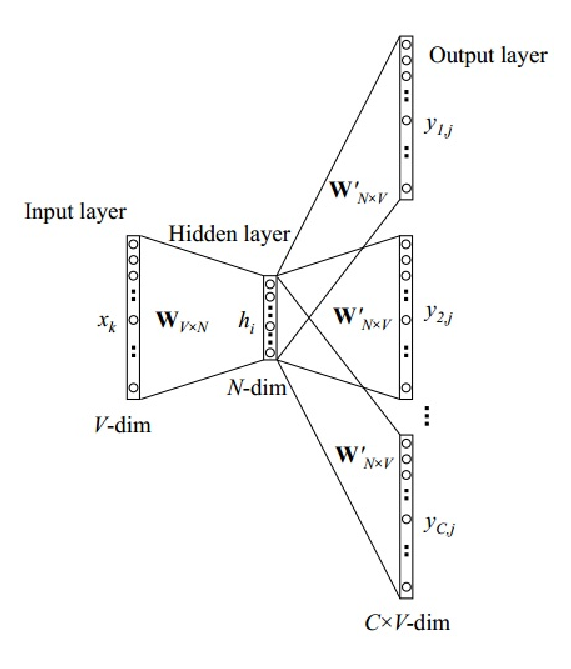
\includegraphics[width=90mm, height=90mm]{skipgram.eps}
\caption{Skip Gram Model(Figure from Rong (2014)) \label{fig:skipgram}}
\end{figure}
The main advantage of using skip-gram is that it is computationally less expensive than other neural language models with a complexity of O(log V) instead of O(V). They use hierarchical softmax~\cite{Morin:05} to achieve such computational efficiency.

\subsection{tf-idf}
\label{subsec:tfidf}
Let $D=d_1, d_2, d_3....d_N$ be $N$ documents under study and $T=t_1, t_2, t_3,....t_M$ be the $M$ unique terms in these documents, then each document can be represented as a $M$-dimensional vector:\\
$t_d=\{tf_1,tf_2,tf_3,...tf_M\}$\\
$tf-idf$ weights discounts the frequency of terms based on their importance to a particular document in the entire document set collection under consideration. This is done as follows:
\begin{center}
$tfidf(d,t)=tf(d,t) \times \log(\frac{|D|}{df(t)})$ 
\end{center}
Here $df(t)$ is the number of documents in which term $t$ appears.

\subsection{Vector Averaging for phrases}
\label{sec:vectoraveraging}
We will describe the process for Hindi but the same flow was followed for English as well.
As an output of the word vector learning, we now have a $n$-dimensional
vector representation for each word in the Hindi corpus.  Now we need to
assign features for sentences and paragraphs taken from the sentiment dataset
(training and test).  Mikolov et al. (2013b) and Levy et al. (2014) show that
many relational similarities can be recovered by means of vector arithmetic
in the embedded space.  Thus, additive models are useful, though
others have claimed that multiplicative models correlate better with human
judgments~\cite{Mitchell:08,Socher:13}.  In this work, we have retained the
simplicity of vector averaging to model larger chunks of  discourse.
This models the sentence/document in the same high dimensional space.

A preprocessing step involved removing some words that appear at very high or
very low frequencies in the corpus.  
Our model was trained on the Hindi Wikipedia dump to create vector
representations for words. The previous two vectors were concatenated to
create another feature set for training purpose.  
%?? SIZE of wikipedia corpus, number of independent words etc. 

\underline{\emph{Algorithm}}
\begin{enumerate}
%\setlength{\itemsep}{0.5pt}
\item Input the Hindi text corpus
\item Train skip-gram model to obtain word vector representation
\item Given a sentiment training set, obtain average vector data for each sentence/document
\item Obtain tf-idf vector for each sentence/document in the corpus
\item Concatenate vectors of step 3 and step 4 to obtain a feature set for a training instance
\item Train linear SVM with $m$-fold cross validation to create a classifier
(here $m$=20)
\end{enumerate}

\section{Document Vectors}
This distributed representation of sentences and documents~\cite{Le:14} modifies word2vec (Skip-Gram) algorithm to unsupervised learning of continuous representations for larger blocks of text, such as sentences, paragraphs or entire documents. The algorithm represents each document by a dense vector which is later trained and tuned to predict words in the sentence\/document.\\
In Paragraph Vector framework, every paragraph is mapped to a unique vector and id, represented by a matrix $D$, which is a column matrix. Every word is mapped to a unique vector and word vectors are concatenated or averaged to predict the context, i.e., the next word.\\
The change in this framework is that the $h$(in Skip-Gram model's equation) is now constructed in a different way. It is now constructed using both $W$ and $D$.\\
The contexts are fixed-length and sampled from a sliding window over the paragraph. The paragraph vector is shared across all contexts generated from the same paragraph but not across paragraphs.  The word vector matrix W, however, is shared across paragraphs. i.e., the vector for "good" is the same for all paragraphs.\\

The paragraph vectors and word vectors are trained using stochastic gradient descent and the gradient is obtained via backpropagation.  At every step of stochastic gradient descent, one can sample a fixed-length context from a random paragraph, compute the error gradient from the network in Figure \ref{fig:doc2vec} and use the gradient to update the parameters in our model. At prediction time, one needs to perform an inference step to compute the paragraph vector for a new paragraph. This is also obtained by gradient descent.  In this step, the parameters for the rest of the model, the word vectors W
and the softmax weights, are fixed.

\begin{figure}[ht!]
\centering
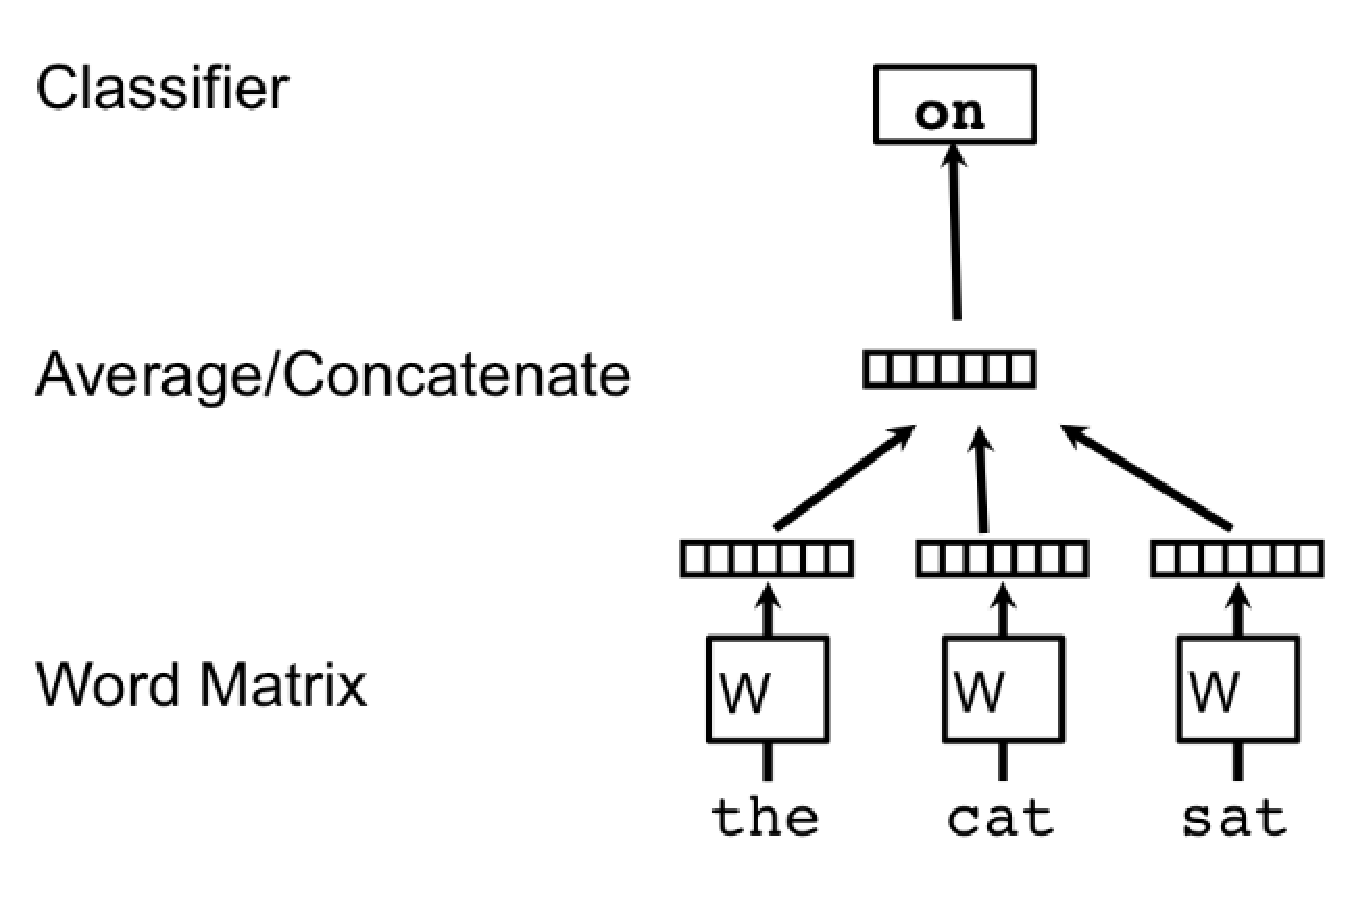
\includegraphics[width=110mm, height=70mm]{doc2vec_word_vector.eps}
\caption{Framework for learning word vectors(Figure from Le (2014)). \label{fig:word2vec}}
\end{figure}
In Figure \ref{fig:word2vec}, context  of three words ("the", "cat" and "sat") is used to predict the fourth word ("on"). The input words are mapped to columns of the matrix $W$ to predict the output word(Figure from Le (2014)).

\begin{figure}[ht!]
\centering
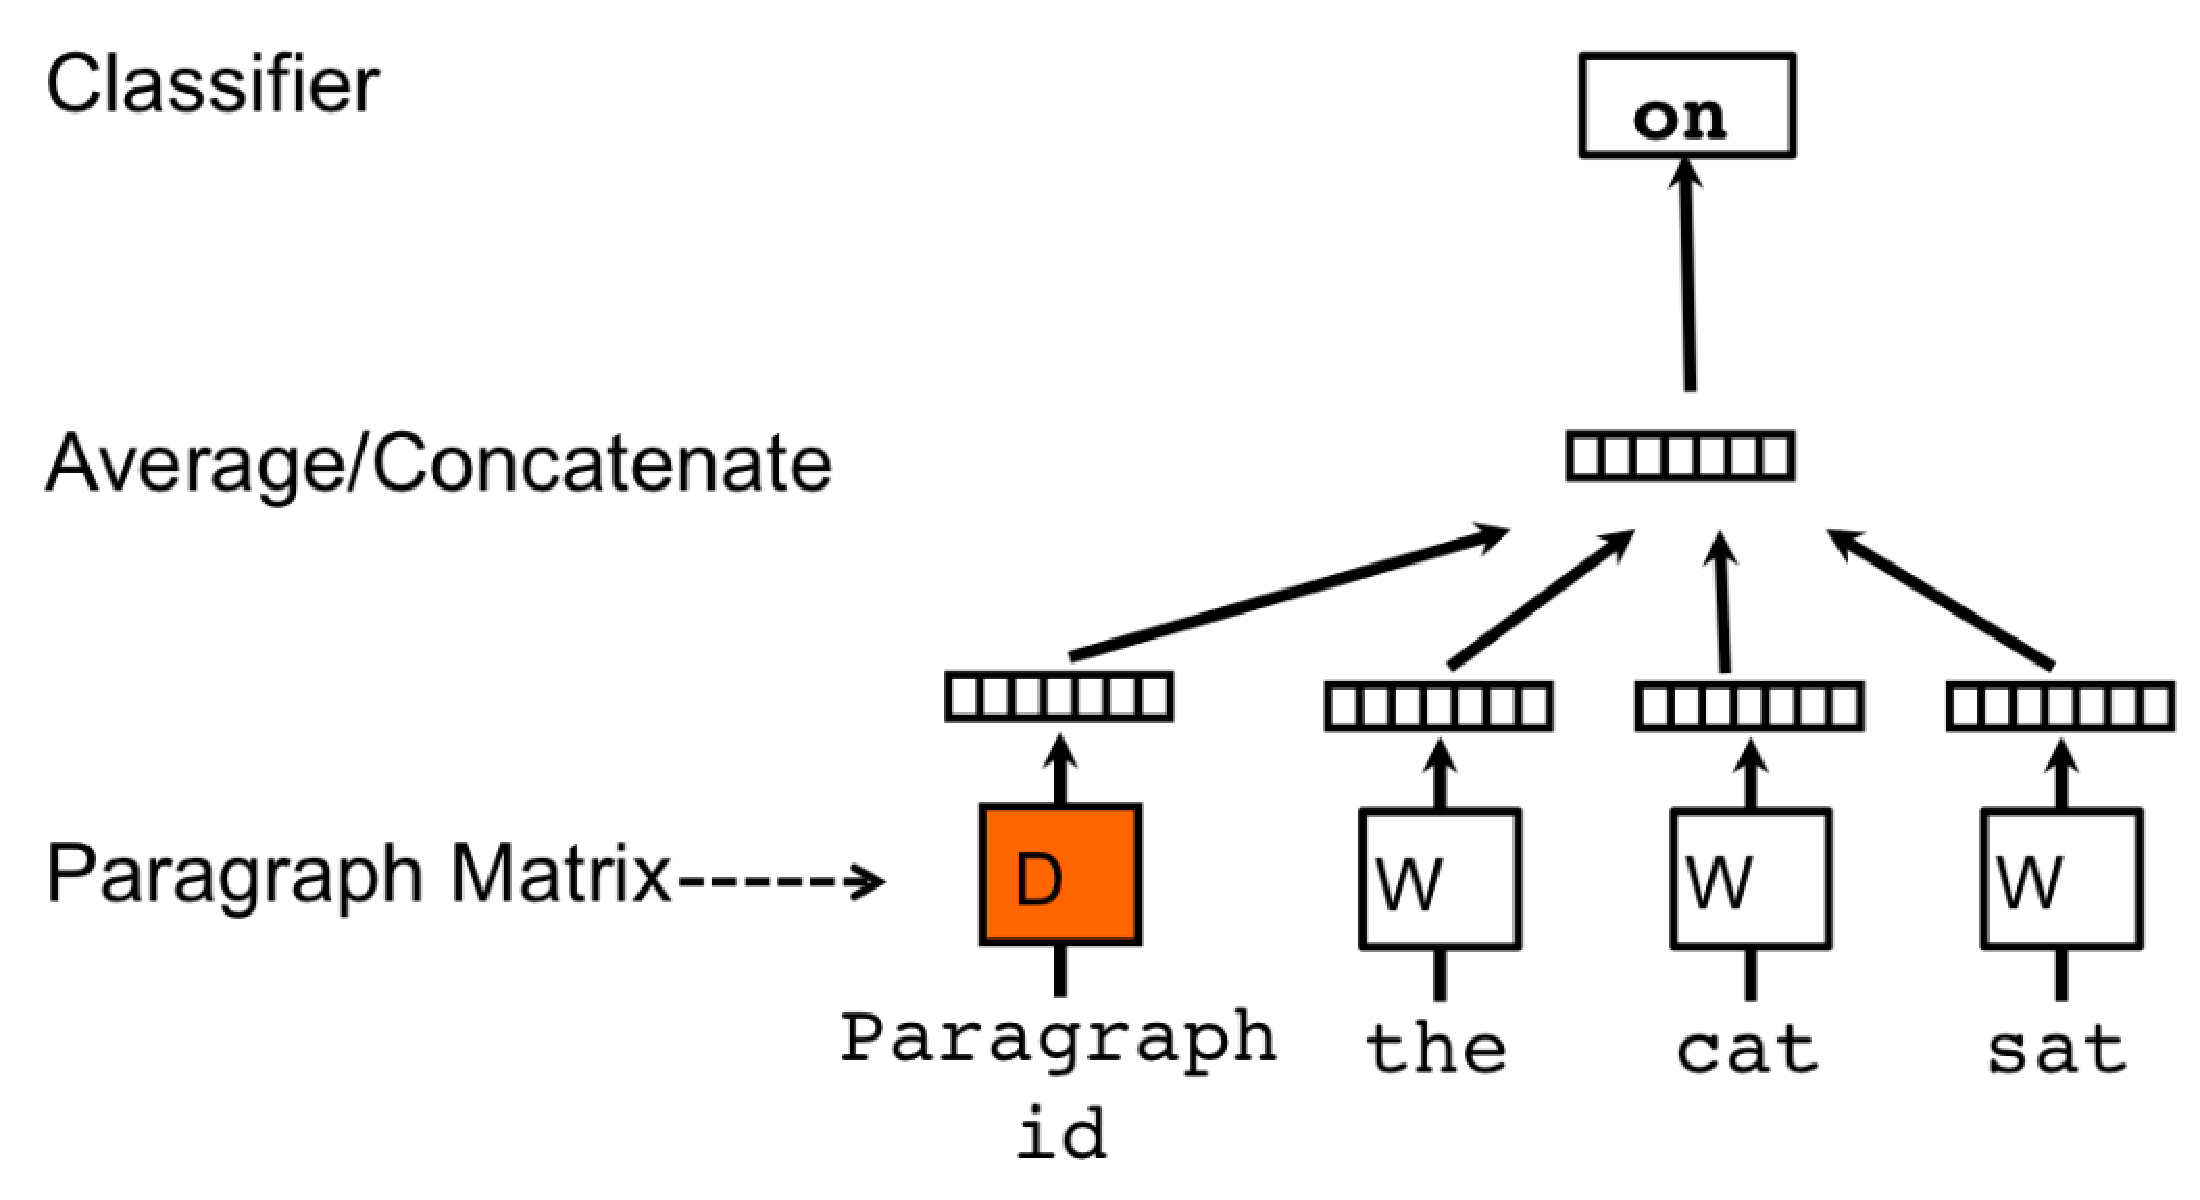
\includegraphics[width=110mm, height=70mm]{doc2vec.eps}
\caption{Framework for learning paragraph vectors(Figure from Le (2014)). \label{fig:doc2vec}}
\end{figure}
In Figure \ref{fig:doc2vec}, the only change is the additional paragraph token that is mapped to a vector via matrix $D$. In this model, the concatenation or average of this vector with a context of three words is used to predict the fourth word. The paragraph vector represents the missing information from the current context and can act as a memory of the topic of the paragraph.

The advantage of using paragraph vectors is that they inherit the property of word vectors, i.e., the semantics of the words. In addition, they also take into consideration a small context around each word which is in close resemblance to the n-gram model with a large n. This property is crucial because the n-gram model preserves a lot of information of the sentence/paragraph, which includes the word order also. This model also performs better than the Bag-of-Words model which would create a very high-dimensional representation that has very poor generalization.

\section{Recurrent Neural Network}
\label{sec:rnn}
The primary feature of a Recurrent Network is that it contains atleast one feed-back connection which captures dynamic temporal behavior and allows it to learn sequences. They have application in tasks such as prediction of a word given the context, perform sequence recognition/reproduction.\\
Recurrent Neural Networks have many different forms. One of them is a Fully Recurrent Network, a network of neuron-like units, each with a directed connection to every other unit.\\
\begin{figure}[ht!]
\centering
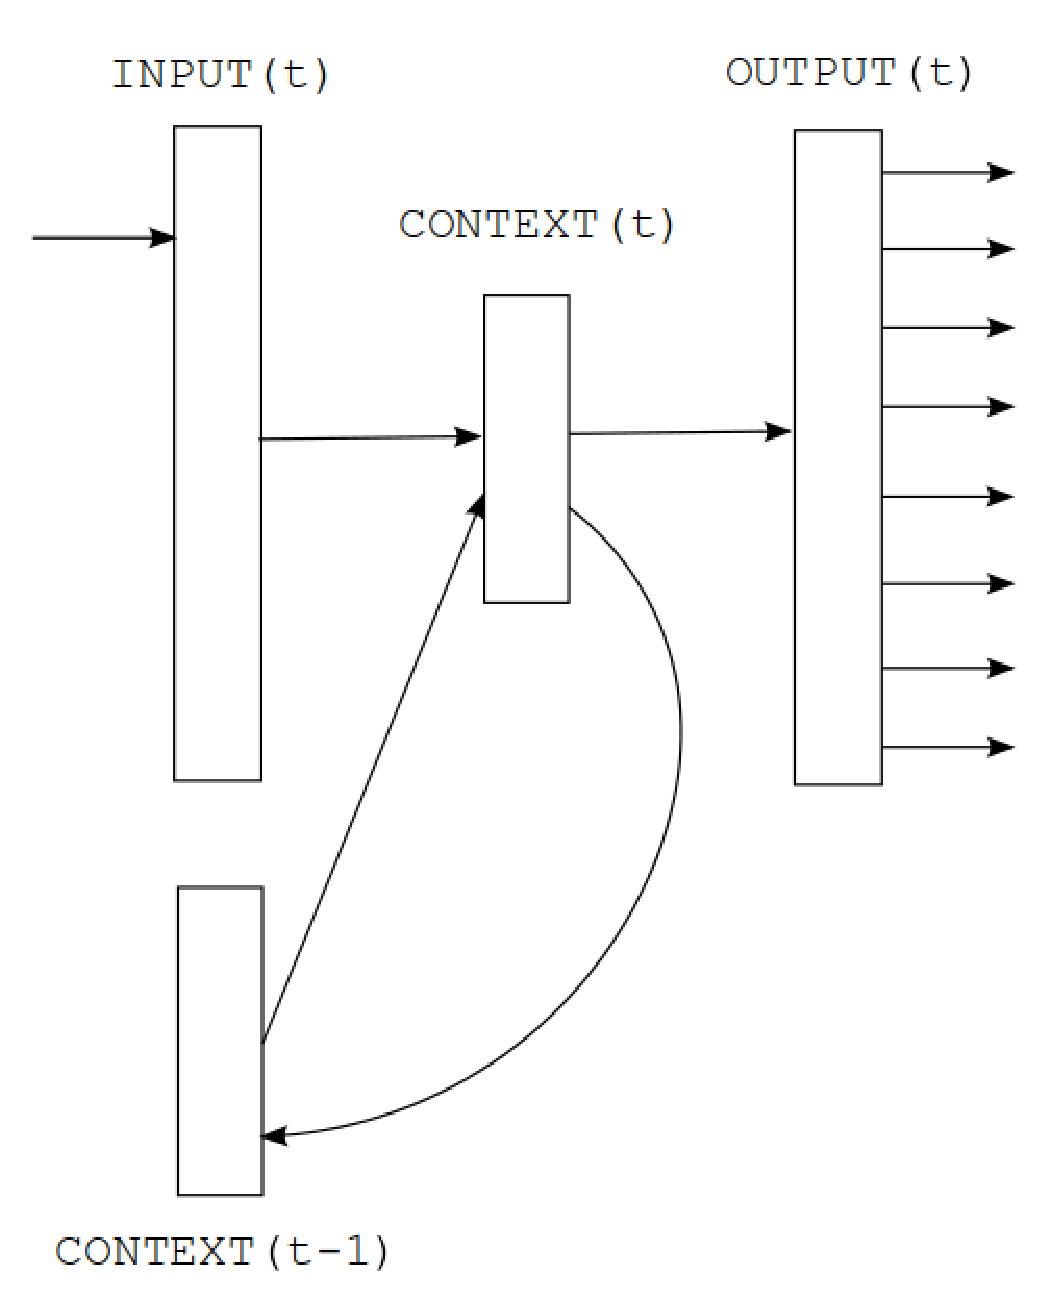
\includegraphics[width=70mm, height=70mm]{rnn.eps}
\caption{Simple Recurrent Neural Network(Figure from \cite{Mikolov:10}). \label{fig:rnn}}
\end{figure}

The architecture of a simple RNN consists of an input layer $x$, a hidden layer $s$(also known as context layer or network state) and an output layer $y$. Since the training is time dependent, we will denote input $x$ as $x(t)$, output $y$ as $y(t)$ and state $s$ as $s(t)$. Input vector $x(t)$ is a concatenation of vector $w$ representing current word, and output from neurons in context layer $s$ at time $t-1$(We can also include output from context layer before $t-1$ as well). The equations of each layer are described below:
\begin{align}
x(t) = w(t) + s(t-1) \\
s_j(t) = f\bigg(\sum_{i}x_i(t)u_{ji}\bigg) \\
y_k(t) = g\bigg(\sum_{j}s_j(t)v_{kj}\bigg)
\end{align}
where $f(z)$ is sigmoid function for activation and $g(z)$ is a softmax function for output prediction:
\begin{align}
f(z) = \frac{1}{1+\mathrm{e}^{-z}} \\
g(z_m) = \frac{\mathrm{e}^{z_m}}{\sum_{k}\mathrm{e}^{z_k}}
\end{align}

\cite{Mikolov:10} claim that size of hidden layer reflects amount of training data with smaller size leading to less number of layers. Weights are initialized to random small values and updated using gradient descent. Output layer $y(t)$ represents probability distribution of next word given previous word $w(t)$ and context $s(t-1)$. The objective function is:
\begin{align}
error(t) =  actual(t) - y(t)
\end{align}
where $actual(t)$ is a $1$-hot vector representing the word that should have been predicted given the context.
\begin {table}[h!]
\centering
\begin{tabular}{ |c|c|c| }
\hline
Model & DEV WER & EVAL WER \\ \hline
Lattice 1 best & 12.9 & 18.4 \\ 
Baseline-KN5 (37M) & 12.2 & 17.2 \\
Discriminative LM (37M) & 11.5 & 16.9 \\
Joint LM (70M) (37M) & - & 16.7 \\ \hline
Static 3xRNN + KN5 (37M) & 11.0 & 15.5 \\
Dynamic 3xRNN + KN5 (37M) & 10.7 & 16.3 \\
\hline
\end{tabular}
\caption {Comparison of WSJ results obtained with various models(RNN is trained on just 6.4M words)}
\label{table:rnn}
\end{table}
Table \ref{table:rnn} represents results of \cite{Mikolov:10} obtained in WSJ experiments using RNN.\\

\cite{Mikolov:11} present several modifications of the original recurrent neural network language model (RNN LM). The present approaches that lead to more than 15 times speedup for both training and testing phases. They also show the importance of backpropagation through time(BPTT) which is an extension to backpropagation algorithm for recurrent networks. With truncated BPTT, the error is propagated through recurrent connections back in time for a specific number of time steps. Thus, the network learns to remember information for several time steps in the hidden layer when it is learned by the BPTT.\\
The speedup is obtained by assuming that words can be mapped to classes. Thus if we assume that each word belongs to exactly one class, we can first estimate the probability distribution over each class using RNN and then calculate the probability of a particular word from the desired class assuming unigram distribution of words within the class. Thus, now we are reducing the connections between hidden and output layer from $V$ to $C$ which is a significant improvement.\\
They are often very sensitive to small changes in its parameters which changes the gradient by a large amount. Few others are, Bi-directional RNN and Hierarchical RNN.\\

\section{Semantic Composition}
\label{sec:composition}
The Principle of Compositionality is that meaning of a complex expression is determined by the meaning of its parts or constituents and the rules which guide this combination. It is also known as \emph{Frege's Principle}. In our case, the constituents are word vectors and the expression in hand is the sentence/document vector. For example,
\begin{center}
\emph{The movie is funny and the screenplay is good}
\end{center}
In the above sentence, consider the word vectors are represented by $w(x)$ and the sentence vector as $S(x)$. Hence,
\begin{align}
S(x) = c_1w_1(x) \Theta c_2w_2(x) \Theta c_3w_3(x) \Theta c_4w_4(x) \dots \Theta c_kw_k(x)
\end{align}
where $\Theta$ can be any operation(e.g., addition, multiplication) and $c_i$s are constants.

\begin {table}[h!]
\centering
\begin{tabular}{ |c|c| }
\hline
Composition & Accuracy \\ \hline \hline
Average & 88.42 \\ \hline
Weighted Average & 88.41 \\ \hline
Multiplication & 50.30 \\ \hline
\end{tabular}
\caption {Results of Vector Composition with different Operations}
\label{table:composition}
\end{table}
Analyzing the results from Table \ref{table:composition}, we observed that when we deal with large number of features, there is a presence of large number of \emph{zeros} and presence of a single zero in a feature will make that features contribution zero in the final vector, which happens in our case and thus multiplicative composition fails.\\
We, therefore, adopt both simple and weighted average methods in our work. The advantage with addition is that, it doesnot increase the dimension of the vector and captures high level semantics with ease. In fact, \cite{Zou:13} have used simple average to construct phrase vectors which they have later used to find phrase level similarity using cosine distance.\\
\cite{Mikolov:13c} showed that relations between words are reflected to a large extent in the offsets between their vector embeddings. They also use additive composition to reflect semantic dependencies.
\begin{center}
\emph{queen - king $\approx$ woman - man}
\end{center}
\cite{Blacoe:12} clearly show that vectors of Neural Language Model and Distributed Model when used with additive composition outperform those with multiplicative composition in Paraphrase Classification task. DM vectors outperform by nearly giving accuracy difference of 6\%. They also perform very well on Phrase similarity tasks.\\
\cite{Socher:13} also present yet another model for semantic composition but that uses a sentiment treebank which is a very costly structure to build and it is task dependent. For under-resourced languages such as Hindi, it would take years to build (for English, task done through Amazon Mechanical Turk). This leads to appreciation of models such as Additive Composition.\\
\begin{figure}[H]
\centering
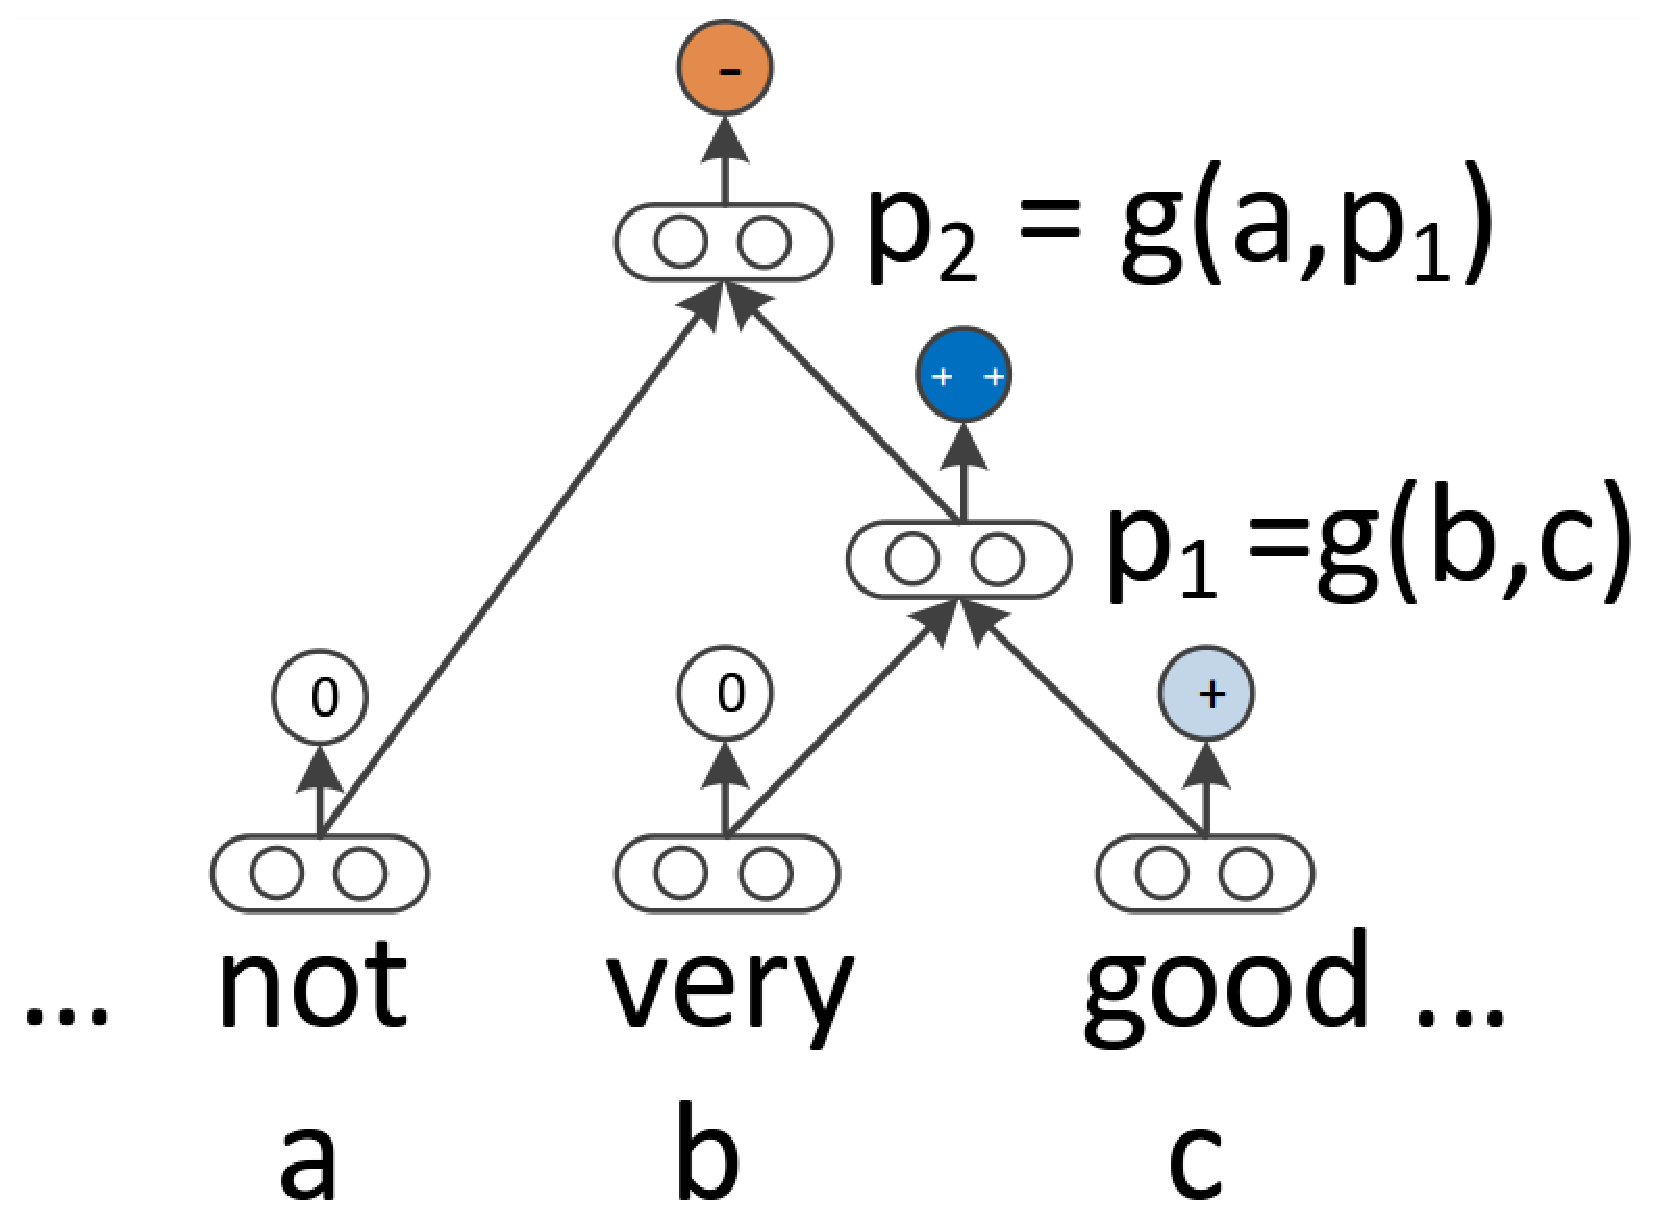
\includegraphics[width=90mm, height=80mm]{recursiveNN.eps}
\caption{Approach of Recursive Neural Network(Figure from \cite{Socher:13}). \label{fig:recursiveNN}}
\end{figure}
Figure \ref{fig:recursiveNN} depicts the approach of recursive neural network. When an n-gram is given to the compositional models, it is parsed into a binary tree and each leaf node, corresponding to a word, is represented as a vector. Recursive neural models will then  compute parent vectors in a bottom up fashion using different types of compositionality functions $g$. The parent vectors are again given as features to a classifier.


\chapter{Conclusions}

In this thesis, we have presented a new SMT interface called \texttt{z3.rkt},
which lets Racket programmers interact with an SMT solver programmatically. We
have demonstrated through examples the simplicity and usefulness of such an
interaction. The power of \texttt{z3.rkt} comes from the facilities provided
by Racket to build abstractions on top of the SMT-solving capabilities of Z3.
From the user's perspective, the integration is seamless and fully
transparent.

Our implementation is open source and freely available at
\begin{center}
\url{http://www.cse.iitk.ac.in/users/karkare/code/z3.rkt/}
\end{center}

\section{Scope for further work}

\texttt{z3.rkt}, like all large projects, is a work in progress. What has been
implemented as of the writing of this thesis is a useful subset of Z3
functionality, but there are several gaps still to be filled:

\begin{itemize}
\item Supporting more Z3 constructs, including bit-vectors and external theories
\item Deriving new abstractions guided by practical use cases
\item Possibly integrating with other SMT solvers
\end{itemize}

In the long term, we hope the community will find this system useful and will
contribute to the project to solve large practical problems.


\begin{singlespace}
\cleardoublepage
\phantomsection \label{listoffig}
\addcontentsline{toc}{chapter}{References}
\renewcommand\bibname{References}
\printbibliography
\nocite{*}
\end{singlespace}

\end{document}
